\documentclass[12pt]{article}
\usepackage{homework}
\pagestyle{fancy}

% assignment information
\def\course{Thermodynamics}
\def\assignmentno{Problem Set 1}
\def\assignmentname{Basic Concepts}
\def\name{Xin, Wenkang}
\def\time{\today}

\begin{document}

\begin{titlepage}
    \begin{center}
        \large
        \textbf{\course}

        \vfill

        \Huge
        \textbf{\assignmentno}

        \vspace{1.5cm}

        \large{\assignmentname}

        \vfill

        \large
        \name

        \time
    \end{center}
\end{titlepage}


%==========
\pagebreak
\section*{Terminology and Some Concepts}
%==========


\problem{A.1}{}
Given that $t \propto V^{2/3}$, we have:

\begin{equation}
    t = \left[ \frac{(10^{-6})^{3}}{10^3} \right]^{2/3} \times \qty{10}{s} = \qty{1}{ms}
\end{equation}
\qed


\problem{A.2}{}
A quasistatic process is one carried out so slowly that the system stays in thermodynamic equilibrium at all times. A process that is quasistatic and has no hysteresis is said to be reversible.

Osmosis and digestion may be taken as quasistatic as they happen slowly over a long period of time.
\qed


\problem{A.3}{}

\begin{table}[h]
    \centering
    \begin{tabular}{|c|c|c|c|c|}
        \hline
        Process & Quasistatic & Reversible & Irreversible & Isothermal \\ \hline
        (a)     & \checkmark  & \checkmark &              &            \\ \hline
        (b)     &             &            & \checkmark   &            \\ \hline
        (c)     & \checkmark  &            & \checkmark   & \checkmark \\ \hline
        (d)     & \checkmark  &            & \mistake{\checkmark}   & \checkmark \\ \hline
        (e)     &             &            & \checkmark   &            \\ \hline
    \end{tabular}
\end{table}

\begin{correction}
    Phase transitions are reversible processes if they happen very slowly.
\end{correction}
\qed


\problem{A.4}{}
A solid has a higher bulk modulus than a gas.

Given the van der Waals equation of state:

\begin{equation}
    \mistake{\left( P + \frac{a}{V^{2}} \right) (V - nb) = nRT}
\end{equation}

At the limit $V \gg nb$, the equation of state reduces to:

\begin{equation}
    V = \frac{nRT}{P + an^{2}/V^{2}}
\end{equation}

so that the bulk modulus is:

\begin{equation}
    \beta = -V \left( \frac{\partial V}{\partial P} \right)_{T} = \left( P + \frac{an^{2}}{V^{2}} \right)^{-1}
\end{equation}

\begin{correction}
    \begin{equation}
        \left( P + \frac{n^{2}a}{V^{2}} \right) (V - nb) = nRT
    \end{equation}

    so that in the limit $V \gg nb$:

    \begin{equation}
        P = \frac{nRT}{V} - \frac{n^{2}a}{V^{2}}
    \end{equation}

    and the bulk modulus is:

    \begin{equation}
        \beta = -V \left( \frac{\partial P}{\partial V} \right)_{T} = \frac{nRT}{V} - \frac{2n^{2}a}{V^{2}}
    \end{equation}
\end{correction}
\qed


\problem{A.5}{Function of state}
Quantities that are functions of state are (a), (b), \mistake{(c)}, (d) and (g).

\begin{correction}
    Quantities that are functions of state are (a), (b), (d) and (g).
\end{correction}
\qed


\problem{A.6}{}
(f) will be an additional function of state, as it is always zero.
\qed


\problem{A.7}{}
We are given a microscopic equation of state:

\begin{equation}
    \left( P + \frac{a}{V^{2}} + \frac{d}{V^{3}} \right) \left( V - b + \frac{f}{V} \right) = RT
\end{equation}

Temperature and pressure are intensive variables that do not change if we change the number of moles of gas. However the volume does change. Consider the distinction between the ideal gas equation in its microscopic and macroscopic forms:

\begin{equation}
\begin{split}
    PV &= RT \\
    PV &= nRT
\end{split}
\end{equation}

We therefore consider the change of variable $V \to V/n$, so that the equation of state becomes:

\begin{equation}
    \left( P + \frac{an^{2}}{V^{2}} + \frac{dn^{3}}{V^{3}} \right) \left( \frac{V}{n} - b + \frac{fn}{V} \right) = RT
\end{equation}
\qed


%==========
\pagebreak
\section*{Partial Math}
%==========


\problem{B.1}{}

\subproblem{a}
Along the first path:

\begin{equation}
\begin{split}
    \int_{(0, 0)}^{(0, 1)} y^{2} \, \mathrm{d}x + xy \, \mathrm{d}y &= 0 \\
    \int_{(0, 1)}^{(1, 1)} y^{2} \, \mathrm{d}x + xy \, \mathrm{d}y &= \int_{0}^{1} 1 \, \mathrm{d}x = 1
\end{split}
\end{equation}

so the integral evaluates to unity.

Along the second path, we have $x = y$ so that:

\begin{equation}
    \int_{(0, 0)}^{(1, 1)} y^{2} \, \mathrm{d}x + xy \, \mathrm{d}y = \int_{0}^{1} 2x^{2} \, \mathrm{d}x = \frac{2}{3}
\end{equation}

This is expected as the integrand is not an exact differential. Check:

\begin{equation}
    \frac{\partial}{\partial y} (y^{2} + xy) = 2y + x \neq \frac{\partial}{\partial x} (y^{2} + xy) = y
\end{equation}

\subproblem{b}
Suppose that the integral is an exact differential $\mathrm{d}\Phi$. Then we need $\partial \Phi/\partial x = y^{2}$ so that:

\begin{equation}
    \Phi = xy^{2} + f(y)
\end{equation}

Differentiating with respect to $y$ gives:

\begin{equation}
    \frac{\partial \Phi}{\partial y} = 2xy + f'(y) = 2xy
\end{equation}

so that $f'(y) = 0$ and $f(y) = C$.

The required function is thus:

\begin{equation}
    \Phi(x, y) = xy^{2} + C
\end{equation}

for some constant $C$.
\qed


\problem{B.2}{}
Check:

\begin{equation}
    \frac{\partial C_{V}}{\partial V} = 0 \ne \frac{\partial (RT/V)}{\partial T} = \frac{R}{V}
\end{equation}

Consider the following quantity instead:

\begin{equation}
    \frac{C_{V}}{T} \, \mathrm{d}T + \frac{R}{V} \, \mathrm{d}V
\end{equation}

We have:

\begin{equation}
    \frac{\partial}{\partial V} \left( \frac{C_{V}}{T} \right) = 0 = \frac{\partial}{\partial T} \left( \frac{R}{V} \right)
\end{equation}

This is an exact differential of the form $\mathrm{d}\Phi$ where:

\begin{equation}
    \Phi = C_{V} \ln{T} + R \ln{V} + C
\end{equation}

for some constant $C$.
\qed


\problem{B.3}{}
Consider some function $f(x, y, z) = C$ for some constant $C$. There are only two independent variables, which we can assume without loss of generality to be $x$ and $y$. Then:

\begin{equation}
\begin{split}
    \mathrm{d}x = \left( \frac{\partial x}{\partial y} \right) \mathrm{d}y + \left( \frac{\partial x}{\partial z} \right) \mathrm{d}z \\
    \mathrm{d}y = \left( \frac{\partial y}{\partial x} \right) \mathrm{d}x + \left( \frac{\partial y}{\partial z} \right) \mathrm{d}z \\
\end{split}
\end{equation}

Substitute the second equation into the first:

\begin{equation}
    \mathrm{d}x = \left( \frac{\partial x}{\partial y} \right) \left[ \left( \frac{\partial y}{\partial x} \right) \mathrm{d}x + \left( \frac{\partial y}{\partial z} \right) \mathrm{d}z \right] + \left( \frac{\partial x}{\partial z} \right) \mathrm{d}z
\end{equation}

From coefficients of $\mathrm{d}x$, we have:

\begin{equation}
    1 = \left( \frac{\partial x}{\partial y} \right) \left( \frac{\partial y}{\partial x} \right)
\end{equation}

From coefficients of $\mathrm{d}z$, we have:

\begin{equation}
    0 = \left( \frac{\partial x}{\partial y} \right) \left( \frac{\partial y}{\partial z} \right) + \left( \frac{\partial x}{\partial z} \right)
\end{equation}

Coupling these two equations gives:

\begin{equation}
    \left( \frac{\partial x}{\partial y} \right) \left( \frac{\partial y}{\partial z} \right) \left( \frac{\partial z}{\partial x} \right) = -1
\end{equation}
\qed


\problem{B.4}{}
Consider a small change in $Q(x, y)$ caused by a small change in $x$ and $y$:

\begin{equation}
    \delta Q = f(x, y) \, \delta x + g(x, y) \, \delta y
\end{equation}

so that:

\begin{equation}
\begin{split}
    \frac{\delta Q}{\delta x} = f(x, y) + g(x, y) \left( \frac{\delta y}{\delta x} \right) \\
    \frac{\delta Q}{\delta y} = f(x, y) \left( \frac{\delta x}{\delta y} \right) + g(x, y)
\end{split}
\end{equation}

Substitute $g(x, y)$ obtained from the second equation into the first:

\begin{equation}
\begin{split}
    \frac{\delta Q}{\delta x} &= f(x, y) + \left[ \frac{\delta Q}{\delta y} - f(x, y) \left( \frac{\delta x}{\delta y} \right) \right] \left( \frac{\delta y}{\delta x} \right) \\
    &= \frac{\delta Q}{\delta y} \left( \frac{\delta y}{\delta x} \right)
\end{split}
\end{equation}

Or, changing to differentials:

\begin{equation}
    \frac{\mathrm{d}Q}{\mathrm{d}x} = \frac{\mathrm{d}Q}{\mathrm{d}y} \left( \frac{\partial y}{\partial x} \right)
\end{equation}

where everything is evaluated at constant points along the path.
\qed


\problem{B.5}{}
In order for $\partial f/\partial x = f/x$ to be true, we must have:

\begin{equation}
    f(x, y, z) = g(y, z) \ln{x}
\end{equation}

for some function $g(y, z)$.
\qed


\problem{B.6}{}
We are given $A = BC$ or:

\begin{equation}
    \mathrm{d}A = C \, \mathrm{d}B
\end{equation}

where we can safely assume a constant $C$ as we will do so later.

Expressing the differentials in terms of variables $x$ and $y$:

\begin{equation}
    \frac{\partial A}{\partial x} \, \mathrm{d}x + \frac{\partial A}{\partial y} \, \mathrm{d}y = C \left( \frac{\partial B}{\partial x} \, \mathrm{d}x + \frac{\partial B}{\partial y} \, \mathrm{d}y \right)
\end{equation}

Collecting terms and dividing both the numerator and denominator by $A$:

\begin{equation}
\begin{split}
    \frac{\mathrm{d}x}{\mathrm{d}y} &= \frac{\partial A/\partial y - C \partial B/\partial y}{\partial A/\partial x - C \partial B/\partial x} \\
    &= \frac{(\partial A/\partial y)/A - (\partial B/\partial y)/B}{(\partial A/\partial x)/A - (\partial B/\partial x)/B} \\
    &= \frac{\partial \ln{A}/\partial y - \partial \ln{B}/\partial y}{\partial \ln{A}/\partial x - \partial \ln{B}/\partial x} \\
\end{split}
\end{equation}

as required.
\qed


%==========
\pagebreak
\section*{Temperature}
%==========


\problem{C.1}{}
Consider the van der Waals equation of state and the ideal gas equation of state, with temperature as the subject:

\begin{equation}
    \begin{split}
        T_{v} &= \frac{V - nb}{nR} P + n^{2}a \left( \frac{1}{V} - \frac{nb}{V^{2}} \right) \\
        T_{i} &= \frac{V}{nR} P
    \end{split}
\end{equation}

In both cases, the temperature is a linear function of pressure, assuming a constant volume. The calibration of the thermometers is a linear transformation $P \to (kP + \epsilon)$ such that for both $T_{v}$ and $T_{i}$, the transformed temperature is zero for some $P_{0}$ and a hundred for some $P_{100}$.

Once transformed, the two temperatures have exactly the same values at $P_{0}$ and $P_{100}$, and the same slope. Therefore, the two temperatures are the same for all pressures.
\qed


\problem{C.2}{}
Write the equation of state as a linear function of pressure:

\begin{equation}
    V = -\kappa V_{0} P + V_{0} (1 + \alpha T)
\end{equation}

The isotherms are straight lines of the same slope $-\kappa V_{0}$ but different intercepts at the $V$-axis.


\begin{figure}[h]
    \centering
    % This file was created with tikzplotlib v0.10.1.
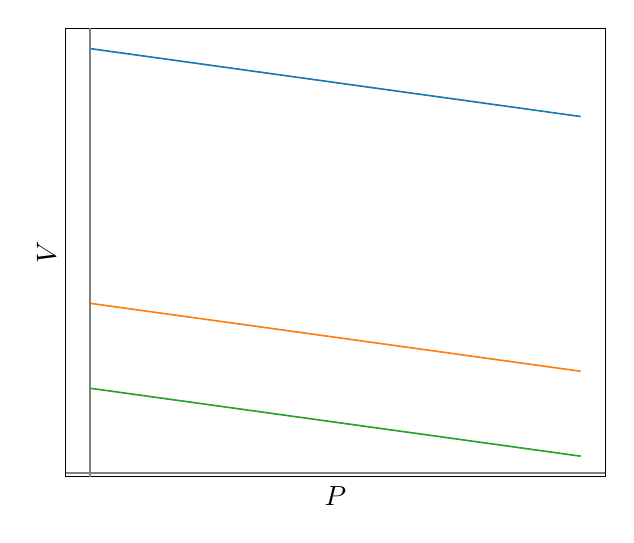
\begin{tikzpicture}

    \definecolor{darkorange25512714}{RGB}{255,127,14}
    \definecolor{forestgreen4416044}{RGB}{44,160,44}
    \definecolor{gray}{RGB}{128,128,128}
    \definecolor{steelblue31119180}{RGB}{31,119,180}
    
    \begin{axis}[
    minor xtick={},
    minor ytick={},
    tick pos=left,
    xlabel={\(\displaystyle P\)},
    xmin=-0.4, xmax=8.4,
    xtick=\empty,
    ylabel={\(\displaystyle V\)},
    ymin=-0.04, ymax=5.24,
    ytick=\empty
    ]
    \addplot [semithick, steelblue31119180]
    table {%
    0 5
    0.0267558528428094 4.99732441471572
    0.0535117056856187 4.99464882943144
    0.0802675585284281 4.99197324414716
    0.107023411371237 4.98929765886288
    0.133779264214047 4.9866220735786
    0.160535117056856 4.98394648829431
    0.187290969899666 4.98127090301003
    0.214046822742475 4.97859531772575
    0.240802675585284 4.97591973244147
    0.267558528428094 4.97324414715719
    0.294314381270903 4.97056856187291
    0.321070234113712 4.96789297658863
    0.347826086956522 4.96521739130435
    0.374581939799331 4.96254180602007
    0.40133779264214 4.95986622073579
    0.42809364548495 4.95719063545151
    0.454849498327759 4.95451505016722
    0.481605351170569 4.95183946488294
    0.508361204013378 4.94916387959866
    0.535117056856187 4.94648829431438
    0.561872909698997 4.9438127090301
    0.588628762541806 4.94113712374582
    0.615384615384615 4.93846153846154
    0.642140468227425 4.93578595317726
    0.668896321070234 4.93311036789298
    0.695652173913043 4.9304347826087
    0.722408026755853 4.92775919732441
    0.749163879598662 4.92508361204013
    0.775919732441472 4.92240802675585
    0.802675585284281 4.91973244147157
    0.82943143812709 4.91705685618729
    0.8561872909699 4.91438127090301
    0.882943143812709 4.91170568561873
    0.909698996655518 4.90903010033445
    0.936454849498328 4.90635451505017
    0.963210702341137 4.90367892976589
    0.989966555183946 4.90100334448161
    1.01672240802676 4.89832775919732
    1.04347826086957 4.89565217391304
    1.07023411371237 4.89297658862876
    1.09698996655518 4.89030100334448
    1.12374581939799 4.8876254180602
    1.1505016722408 4.88494983277592
    1.17725752508361 4.88227424749164
    1.20401337792642 4.87959866220736
    1.23076923076923 4.87692307692308
    1.25752508361204 4.8742474916388
    1.28428093645485 4.87157190635452
    1.31103678929766 4.86889632107023
    1.33779264214047 4.86622073578595
    1.36454849498328 4.86354515050167
    1.39130434782609 4.86086956521739
    1.4180602006689 4.85819397993311
    1.44481605351171 4.85551839464883
    1.47157190635451 4.85284280936455
    1.49832775919732 4.85016722408027
    1.52508361204013 4.84749163879599
    1.55183946488294 4.84481605351171
    1.57859531772575 4.84214046822742
    1.60535117056856 4.83946488294314
    1.63210702341137 4.83678929765886
    1.65886287625418 4.83411371237458
    1.68561872909699 4.8314381270903
    1.7123745819398 4.82876254180602
    1.73913043478261 4.82608695652174
    1.76588628762542 4.82341137123746
    1.79264214046823 4.82073578595318
    1.81939799331104 4.8180602006689
    1.84615384615385 4.81538461538462
    1.87290969899666 4.81270903010033
    1.89966555183946 4.81003344481605
    1.92642140468227 4.80735785953177
    1.95317725752508 4.80468227424749
    1.97993311036789 4.80200668896321
    2.0066889632107 4.79933110367893
    2.03344481605351 4.79665551839465
    2.06020066889632 4.79397993311037
    2.08695652173913 4.79130434782609
    2.11371237458194 4.78862876254181
    2.14046822742475 4.78595317725753
    2.16722408026756 4.78327759197324
    2.19397993311037 4.78060200668896
    2.22073578595318 4.77792642140468
    2.24749163879599 4.7752508361204
    2.2742474916388 4.77257525083612
    2.30100334448161 4.76989966555184
    2.32775919732441 4.76722408026756
    2.35451505016722 4.76454849498328
    2.38127090301003 4.761872909699
    2.40802675585284 4.75919732441472
    2.43478260869565 4.75652173913043
    2.46153846153846 4.75384615384615
    2.48829431438127 4.75117056856187
    2.51505016722408 4.74849498327759
    2.54180602006689 4.74581939799331
    2.5685618729097 4.74314381270903
    2.59531772575251 4.74046822742475
    2.62207357859532 4.73779264214047
    2.64882943143813 4.73511705685619
    2.67558528428094 4.73244147157191
    2.70234113712375 4.72976588628763
    2.72909698996656 4.72709030100334
    2.75585284280936 4.72441471571906
    2.78260869565217 4.72173913043478
    2.80936454849498 4.7190635451505
    2.83612040133779 4.71638795986622
    2.8628762541806 4.71371237458194
    2.88963210702341 4.71103678929766
    2.91638795986622 4.70836120401338
    2.94314381270903 4.7056856187291
    2.96989966555184 4.70301003344482
    2.99665551839465 4.70033444816054
    3.02341137123746 4.69765886287625
    3.05016722408027 4.69498327759197
    3.07692307692308 4.69230769230769
    3.10367892976589 4.68963210702341
    3.1304347826087 4.68695652173913
    3.15719063545151 4.68428093645485
    3.18394648829431 4.68160535117057
    3.21070234113712 4.67892976588629
    3.23745819397993 4.67625418060201
    3.26421404682274 4.67357859531773
    3.29096989966555 4.67090301003345
    3.31772575250836 4.66822742474916
    3.34448160535117 4.66555183946488
    3.37123745819398 4.6628762541806
    3.39799331103679 4.66020066889632
    3.4247491638796 4.65752508361204
    3.45150501672241 4.65484949832776
    3.47826086956522 4.65217391304348
    3.50501672240803 4.6494983277592
    3.53177257525084 4.64682274247492
    3.55852842809365 4.64414715719064
    3.58528428093645 4.64147157190635
    3.61204013377926 4.63879598662207
    3.63879598662207 4.63612040133779
    3.66555183946488 4.63344481605351
    3.69230769230769 4.63076923076923
    3.7190635451505 4.62809364548495
    3.74581939799331 4.62541806020067
    3.77257525083612 4.62274247491639
    3.79933110367893 4.62006688963211
    3.82608695652174 4.61739130434783
    3.85284280936455 4.61471571906355
    3.87959866220736 4.61204013377926
    3.90635451505017 4.60936454849498
    3.93311036789298 4.6066889632107
    3.95986622073579 4.60401337792642
    3.9866220735786 4.60133779264214
    4.0133779264214 4.59866220735786
    4.04013377926421 4.59598662207358
    4.06688963210702 4.5933110367893
    4.09364548494983 4.59063545150502
    4.12040133779264 4.58795986622074
    4.14715719063545 4.58528428093646
    4.17391304347826 4.58260869565217
    4.20066889632107 4.57993311036789
    4.22742474916388 4.57725752508361
    4.25418060200669 4.57458193979933
    4.2809364548495 4.57190635451505
    4.30769230769231 4.56923076923077
    4.33444816053512 4.56655518394649
    4.36120401337793 4.56387959866221
    4.38795986622074 4.56120401337793
    4.41471571906354 4.55852842809365
    4.44147157190635 4.55585284280936
    4.46822742474916 4.55317725752508
    4.49498327759197 4.5505016722408
    4.52173913043478 4.54782608695652
    4.54849498327759 4.54515050167224
    4.5752508361204 4.54247491638796
    4.60200668896321 4.53979933110368
    4.62876254180602 4.5371237458194
    4.65551839464883 4.53444816053512
    4.68227424749164 4.53177257525084
    4.70903010033445 4.52909698996655
    4.73578595317726 4.52642140468227
    4.76254180602007 4.52374581939799
    4.78929765886288 4.52107023411371
    4.81605351170569 4.51839464882943
    4.8428093645485 4.51571906354515
    4.8695652173913 4.51304347826087
    4.89632107023411 4.51036789297659
    4.92307692307692 4.50769230769231
    4.94983277591973 4.50501672240803
    4.97658862876254 4.50234113712375
    5.00334448160535 4.49966555183947
    5.03010033444816 4.49698996655518
    5.05685618729097 4.4943143812709
    5.08361204013378 4.49163879598662
    5.11036789297659 4.48896321070234
    5.1371237458194 4.48628762541806
    5.16387959866221 4.48361204013378
    5.19063545150502 4.4809364548495
    5.21739130434783 4.47826086956522
    5.24414715719064 4.47558528428094
    5.27090301003344 4.47290969899666
    5.29765886287625 4.47023411371237
    5.32441471571906 4.46755852842809
    5.35117056856187 4.46488294314381
    5.37792642140468 4.46220735785953
    5.40468227424749 4.45953177257525
    5.4314381270903 4.45685618729097
    5.45819397993311 4.45418060200669
    5.48494983277592 4.45150501672241
    5.51170568561873 4.44882943143813
    5.53846153846154 4.44615384615385
    5.56521739130435 4.44347826086956
    5.59197324414716 4.44080267558528
    5.61872909698997 4.438127090301
    5.64548494983278 4.43545150501672
    5.67224080267559 4.43277591973244
    5.69899665551839 4.43010033444816
    5.7257525083612 4.42742474916388
    5.75250836120401 4.4247491638796
    5.77926421404682 4.42207357859532
    5.80602006688963 4.41939799331104
    5.83277591973244 4.41672240802676
    5.85953177257525 4.41404682274247
    5.88628762541806 4.41137123745819
    5.91304347826087 4.40869565217391
    5.93979933110368 4.40602006688963
    5.96655518394649 4.40334448160535
    5.9933110367893 4.40066889632107
    6.02006688963211 4.39799331103679
    6.04682274247492 4.39531772575251
    6.07357859531773 4.39264214046823
    6.10033444816053 4.38996655518395
    6.12709030100334 4.38729096989967
    6.15384615384615 4.38461538461539
    6.18060200668896 4.3819397993311
    6.20735785953177 4.37926421404682
    6.23411371237458 4.37658862876254
    6.26086956521739 4.37391304347826
    6.2876254180602 4.37123745819398
    6.31438127090301 4.3685618729097
    6.34113712374582 4.36588628762542
    6.36789297658863 4.36321070234114
    6.39464882943144 4.36053511705686
    6.42140468227425 4.35785953177258
    6.44816053511706 4.35518394648829
    6.47491638795987 4.35250836120401
    6.50167224080268 4.34983277591973
    6.52842809364549 4.34715719063545
    6.55518394648829 4.34448160535117
    6.5819397993311 4.34180602006689
    6.60869565217391 4.33913043478261
    6.63545150501672 4.33645484949833
    6.66220735785953 4.33377926421405
    6.68896321070234 4.33110367892977
    6.71571906354515 4.32842809364548
    6.74247491638796 4.3257525083612
    6.76923076923077 4.32307692307692
    6.79598662207358 4.32040133779264
    6.82274247491639 4.31772575250836
    6.8494983277592 4.31505016722408
    6.87625418060201 4.3123745819398
    6.90301003344482 4.30969899665552
    6.92976588628763 4.30702341137124
    6.95652173913043 4.30434782608696
    6.98327759197324 4.30167224080268
    7.01003344481605 4.29899665551839
    7.03678929765886 4.29632107023411
    7.06354515050167 4.29364548494983
    7.09030100334448 4.29096989966555
    7.11705685618729 4.28829431438127
    7.1438127090301 4.28561872909699
    7.17056856187291 4.28294314381271
    7.19732441471572 4.28026755852843
    7.22408026755853 4.27759197324415
    7.25083612040134 4.27491638795987
    7.27759197324415 4.27224080267559
    7.30434782608696 4.2695652173913
    7.33110367892977 4.26688963210702
    7.35785953177257 4.26421404682274
    7.38461538461538 4.26153846153846
    7.41137123745819 4.25886287625418
    7.438127090301 4.2561872909699
    7.46488294314381 4.25351170568562
    7.49163879598662 4.25083612040134
    7.51839464882943 4.24816053511706
    7.54515050167224 4.24548494983278
    7.57190635451505 4.24280936454849
    7.59866220735786 4.24013377926421
    7.62541806020067 4.23745819397993
    7.65217391304348 4.23478260869565
    7.67892976588629 4.23210702341137
    7.7056856187291 4.22943143812709
    7.73244147157191 4.22675585284281
    7.75919732441472 4.22408026755853
    7.78595317725753 4.22140468227425
    7.81270903010033 4.21872909698997
    7.83946488294314 4.21605351170569
    7.86622073578595 4.2133779264214
    7.89297658862876 4.21070234113712
    7.91973244147157 4.20802675585284
    7.94648829431438 4.20535117056856
    7.97324414715719 4.20267558528428
    8 4.2
    };
    \addplot [semithick, darkorange25512714]
    table {%
    0 2
    0.0267558528428094 1.99732441471572
    0.0535117056856187 1.99464882943144
    0.0802675585284281 1.99197324414716
    0.107023411371237 1.98929765886288
    0.133779264214047 1.9866220735786
    0.160535117056856 1.98394648829431
    0.187290969899666 1.98127090301003
    0.214046822742475 1.97859531772575
    0.240802675585284 1.97591973244147
    0.267558528428094 1.97324414715719
    0.294314381270903 1.97056856187291
    0.321070234113712 1.96789297658863
    0.347826086956522 1.96521739130435
    0.374581939799331 1.96254180602007
    0.40133779264214 1.95986622073579
    0.42809364548495 1.9571906354515
    0.454849498327759 1.95451505016722
    0.481605351170569 1.95183946488294
    0.508361204013378 1.94916387959866
    0.535117056856187 1.94648829431438
    0.561872909698997 1.9438127090301
    0.588628762541806 1.94113712374582
    0.615384615384615 1.93846153846154
    0.642140468227425 1.93578595317726
    0.668896321070234 1.93311036789298
    0.695652173913043 1.9304347826087
    0.722408026755853 1.92775919732441
    0.749163879598662 1.92508361204013
    0.775919732441472 1.92240802675585
    0.802675585284281 1.91973244147157
    0.82943143812709 1.91705685618729
    0.8561872909699 1.91438127090301
    0.882943143812709 1.91170568561873
    0.909698996655518 1.90903010033445
    0.936454849498328 1.90635451505017
    0.963210702341137 1.90367892976589
    0.989966555183946 1.90100334448161
    1.01672240802676 1.89832775919732
    1.04347826086957 1.89565217391304
    1.07023411371237 1.89297658862876
    1.09698996655518 1.89030100334448
    1.12374581939799 1.8876254180602
    1.1505016722408 1.88494983277592
    1.17725752508361 1.88227424749164
    1.20401337792642 1.87959866220736
    1.23076923076923 1.87692307692308
    1.25752508361204 1.8742474916388
    1.28428093645485 1.87157190635452
    1.31103678929766 1.86889632107023
    1.33779264214047 1.86622073578595
    1.36454849498328 1.86354515050167
    1.39130434782609 1.86086956521739
    1.4180602006689 1.85819397993311
    1.44481605351171 1.85551839464883
    1.47157190635451 1.85284280936455
    1.49832775919732 1.85016722408027
    1.52508361204013 1.84749163879599
    1.55183946488294 1.84481605351171
    1.57859531772575 1.84214046822742
    1.60535117056856 1.83946488294314
    1.63210702341137 1.83678929765886
    1.65886287625418 1.83411371237458
    1.68561872909699 1.8314381270903
    1.7123745819398 1.82876254180602
    1.73913043478261 1.82608695652174
    1.76588628762542 1.82341137123746
    1.79264214046823 1.82073578595318
    1.81939799331104 1.8180602006689
    1.84615384615385 1.81538461538462
    1.87290969899666 1.81270903010033
    1.89966555183946 1.81003344481605
    1.92642140468227 1.80735785953177
    1.95317725752508 1.80468227424749
    1.97993311036789 1.80200668896321
    2.0066889632107 1.79933110367893
    2.03344481605351 1.79665551839465
    2.06020066889632 1.79397993311037
    2.08695652173913 1.79130434782609
    2.11371237458194 1.78862876254181
    2.14046822742475 1.78595317725753
    2.16722408026756 1.78327759197324
    2.19397993311037 1.78060200668896
    2.22073578595318 1.77792642140468
    2.24749163879599 1.7752508361204
    2.2742474916388 1.77257525083612
    2.30100334448161 1.76989966555184
    2.32775919732441 1.76722408026756
    2.35451505016722 1.76454849498328
    2.38127090301003 1.761872909699
    2.40802675585284 1.75919732441472
    2.43478260869565 1.75652173913043
    2.46153846153846 1.75384615384615
    2.48829431438127 1.75117056856187
    2.51505016722408 1.74849498327759
    2.54180602006689 1.74581939799331
    2.5685618729097 1.74314381270903
    2.59531772575251 1.74046822742475
    2.62207357859532 1.73779264214047
    2.64882943143813 1.73511705685619
    2.67558528428094 1.73244147157191
    2.70234113712375 1.72976588628763
    2.72909698996656 1.72709030100334
    2.75585284280936 1.72441471571906
    2.78260869565217 1.72173913043478
    2.80936454849498 1.7190635451505
    2.83612040133779 1.71638795986622
    2.8628762541806 1.71371237458194
    2.88963210702341 1.71103678929766
    2.91638795986622 1.70836120401338
    2.94314381270903 1.7056856187291
    2.96989966555184 1.70301003344482
    2.99665551839465 1.70033444816054
    3.02341137123746 1.69765886287625
    3.05016722408027 1.69498327759197
    3.07692307692308 1.69230769230769
    3.10367892976589 1.68963210702341
    3.1304347826087 1.68695652173913
    3.15719063545151 1.68428093645485
    3.18394648829431 1.68160535117057
    3.21070234113712 1.67892976588629
    3.23745819397993 1.67625418060201
    3.26421404682274 1.67357859531773
    3.29096989966555 1.67090301003344
    3.31772575250836 1.66822742474916
    3.34448160535117 1.66555183946488
    3.37123745819398 1.6628762541806
    3.39799331103679 1.66020066889632
    3.4247491638796 1.65752508361204
    3.45150501672241 1.65484949832776
    3.47826086956522 1.65217391304348
    3.50501672240803 1.6494983277592
    3.53177257525084 1.64682274247492
    3.55852842809365 1.64414715719064
    3.58528428093645 1.64147157190635
    3.61204013377926 1.63879598662207
    3.63879598662207 1.63612040133779
    3.66555183946488 1.63344481605351
    3.69230769230769 1.63076923076923
    3.7190635451505 1.62809364548495
    3.74581939799331 1.62541806020067
    3.77257525083612 1.62274247491639
    3.79933110367893 1.62006688963211
    3.82608695652174 1.61739130434783
    3.85284280936455 1.61471571906355
    3.87959866220736 1.61204013377926
    3.90635451505017 1.60936454849498
    3.93311036789298 1.6066889632107
    3.95986622073579 1.60401337792642
    3.9866220735786 1.60133779264214
    4.0133779264214 1.59866220735786
    4.04013377926421 1.59598662207358
    4.06688963210702 1.5933110367893
    4.09364548494983 1.59063545150502
    4.12040133779264 1.58795986622074
    4.14715719063545 1.58528428093645
    4.17391304347826 1.58260869565217
    4.20066889632107 1.57993311036789
    4.22742474916388 1.57725752508361
    4.25418060200669 1.57458193979933
    4.2809364548495 1.57190635451505
    4.30769230769231 1.56923076923077
    4.33444816053512 1.56655518394649
    4.36120401337793 1.56387959866221
    4.38795986622074 1.56120401337793
    4.41471571906354 1.55852842809365
    4.44147157190635 1.55585284280936
    4.46822742474916 1.55317725752508
    4.49498327759197 1.5505016722408
    4.52173913043478 1.54782608695652
    4.54849498327759 1.54515050167224
    4.5752508361204 1.54247491638796
    4.60200668896321 1.53979933110368
    4.62876254180602 1.5371237458194
    4.65551839464883 1.53444816053512
    4.68227424749164 1.53177257525084
    4.70903010033445 1.52909698996656
    4.73578595317726 1.52642140468227
    4.76254180602007 1.52374581939799
    4.78929765886288 1.52107023411371
    4.81605351170569 1.51839464882943
    4.8428093645485 1.51571906354515
    4.8695652173913 1.51304347826087
    4.89632107023411 1.51036789297659
    4.92307692307692 1.50769230769231
    4.94983277591973 1.50501672240803
    4.97658862876254 1.50234113712375
    5.00334448160535 1.49966555183946
    5.03010033444816 1.49698996655518
    5.05685618729097 1.4943143812709
    5.08361204013378 1.49163879598662
    5.11036789297659 1.48896321070234
    5.1371237458194 1.48628762541806
    5.16387959866221 1.48361204013378
    5.19063545150502 1.4809364548495
    5.21739130434783 1.47826086956522
    5.24414715719064 1.47558528428094
    5.27090301003344 1.47290969899666
    5.29765886287625 1.47023411371237
    5.32441471571906 1.46755852842809
    5.35117056856187 1.46488294314381
    5.37792642140468 1.46220735785953
    5.40468227424749 1.45953177257525
    5.4314381270903 1.45685618729097
    5.45819397993311 1.45418060200669
    5.48494983277592 1.45150501672241
    5.51170568561873 1.44882943143813
    5.53846153846154 1.44615384615385
    5.56521739130435 1.44347826086957
    5.59197324414716 1.44080267558528
    5.61872909698997 1.438127090301
    5.64548494983278 1.43545150501672
    5.67224080267559 1.43277591973244
    5.69899665551839 1.43010033444816
    5.7257525083612 1.42742474916388
    5.75250836120401 1.4247491638796
    5.77926421404682 1.42207357859532
    5.80602006688963 1.41939799331104
    5.83277591973244 1.41672240802676
    5.85953177257525 1.41404682274247
    5.88628762541806 1.41137123745819
    5.91304347826087 1.40869565217391
    5.93979933110368 1.40602006688963
    5.96655518394649 1.40334448160535
    5.9933110367893 1.40066889632107
    6.02006688963211 1.39799331103679
    6.04682274247492 1.39531772575251
    6.07357859531773 1.39264214046823
    6.10033444816053 1.38996655518395
    6.12709030100334 1.38729096989967
    6.15384615384615 1.38461538461538
    6.18060200668896 1.3819397993311
    6.20735785953177 1.37926421404682
    6.23411371237458 1.37658862876254
    6.26086956521739 1.37391304347826
    6.2876254180602 1.37123745819398
    6.31438127090301 1.3685618729097
    6.34113712374582 1.36588628762542
    6.36789297658863 1.36321070234114
    6.39464882943144 1.36053511705686
    6.42140468227425 1.35785953177258
    6.44816053511706 1.35518394648829
    6.47491638795987 1.35250836120401
    6.50167224080268 1.34983277591973
    6.52842809364549 1.34715719063545
    6.55518394648829 1.34448160535117
    6.5819397993311 1.34180602006689
    6.60869565217391 1.33913043478261
    6.63545150501672 1.33645484949833
    6.66220735785953 1.33377926421405
    6.68896321070234 1.33110367892977
    6.71571906354515 1.32842809364548
    6.74247491638796 1.3257525083612
    6.76923076923077 1.32307692307692
    6.79598662207358 1.32040133779264
    6.82274247491639 1.31772575250836
    6.8494983277592 1.31505016722408
    6.87625418060201 1.3123745819398
    6.90301003344482 1.30969899665552
    6.92976588628763 1.30702341137124
    6.95652173913043 1.30434782608696
    6.98327759197324 1.30167224080268
    7.01003344481605 1.29899665551839
    7.03678929765886 1.29632107023411
    7.06354515050167 1.29364548494983
    7.09030100334448 1.29096989966555
    7.11705685618729 1.28829431438127
    7.1438127090301 1.28561872909699
    7.17056856187291 1.28294314381271
    7.19732441471572 1.28026755852843
    7.22408026755853 1.27759197324415
    7.25083612040134 1.27491638795987
    7.27759197324415 1.27224080267559
    7.30434782608696 1.2695652173913
    7.33110367892977 1.26688963210702
    7.35785953177257 1.26421404682274
    7.38461538461538 1.26153846153846
    7.41137123745819 1.25886287625418
    7.438127090301 1.2561872909699
    7.46488294314381 1.25351170568562
    7.49163879598662 1.25083612040134
    7.51839464882943 1.24816053511706
    7.54515050167224 1.24548494983278
    7.57190635451505 1.24280936454849
    7.59866220735786 1.24013377926421
    7.62541806020067 1.23745819397993
    7.65217391304348 1.23478260869565
    7.67892976588629 1.23210702341137
    7.7056856187291 1.22943143812709
    7.73244147157191 1.22675585284281
    7.75919732441472 1.22408026755853
    7.78595317725753 1.22140468227425
    7.81270903010033 1.21872909698997
    7.83946488294314 1.21605351170569
    7.86622073578595 1.2133779264214
    7.89297658862876 1.21070234113712
    7.91973244147157 1.20802675585284
    7.94648829431438 1.20535117056856
    7.97324414715719 1.20267558528428
    8 1.2
    };
    \addplot [semithick, forestgreen4416044]
    table {%
    0 1
    0.0267558528428094 0.997324414715719
    0.0535117056856187 0.994648829431438
    0.0802675585284281 0.991973244147157
    0.107023411371237 0.989297658862876
    0.133779264214047 0.986622073578595
    0.160535117056856 0.983946488294314
    0.187290969899666 0.981270903010034
    0.214046822742475 0.978595317725752
    0.240802675585284 0.975919732441472
    0.267558528428094 0.973244147157191
    0.294314381270903 0.97056856187291
    0.321070234113712 0.967892976588629
    0.347826086956522 0.965217391304348
    0.374581939799331 0.962541806020067
    0.40133779264214 0.959866220735786
    0.42809364548495 0.957190635451505
    0.454849498327759 0.954515050167224
    0.481605351170569 0.951839464882943
    0.508361204013378 0.949163879598662
    0.535117056856187 0.946488294314381
    0.561872909698997 0.9438127090301
    0.588628762541806 0.941137123745819
    0.615384615384615 0.938461538461538
    0.642140468227425 0.935785953177258
    0.668896321070234 0.933110367892977
    0.695652173913043 0.930434782608696
    0.722408026755853 0.927759197324415
    0.749163879598662 0.925083612040134
    0.775919732441472 0.922408026755853
    0.802675585284281 0.919732441471572
    0.82943143812709 0.917056856187291
    0.8561872909699 0.91438127090301
    0.882943143812709 0.911705685618729
    0.909698996655518 0.909030100334448
    0.936454849498328 0.906354515050167
    0.963210702341137 0.903678929765886
    0.989966555183946 0.901003344481605
    1.01672240802676 0.898327759197324
    1.04347826086957 0.895652173913043
    1.07023411371237 0.892976588628763
    1.09698996655518 0.890301003344482
    1.12374581939799 0.887625418060201
    1.1505016722408 0.88494983277592
    1.17725752508361 0.882274247491639
    1.20401337792642 0.879598662207358
    1.23076923076923 0.876923076923077
    1.25752508361204 0.874247491638796
    1.28428093645485 0.871571906354515
    1.31103678929766 0.868896321070234
    1.33779264214047 0.866220735785953
    1.36454849498328 0.863545150501672
    1.39130434782609 0.860869565217391
    1.4180602006689 0.85819397993311
    1.44481605351171 0.855518394648829
    1.47157190635451 0.852842809364548
    1.49832775919732 0.850167224080268
    1.52508361204013 0.847491638795987
    1.55183946488294 0.844816053511706
    1.57859531772575 0.842140468227425
    1.60535117056856 0.839464882943144
    1.63210702341137 0.836789297658863
    1.65886287625418 0.834113712374582
    1.68561872909699 0.831438127090301
    1.7123745819398 0.82876254180602
    1.73913043478261 0.826086956521739
    1.76588628762542 0.823411371237458
    1.79264214046823 0.820735785953177
    1.81939799331104 0.818060200668896
    1.84615384615385 0.815384615384615
    1.87290969899666 0.812709030100334
    1.89966555183946 0.810033444816054
    1.92642140468227 0.807357859531773
    1.95317725752508 0.804682274247492
    1.97993311036789 0.802006688963211
    2.0066889632107 0.79933110367893
    2.03344481605351 0.796655518394649
    2.06020066889632 0.793979933110368
    2.08695652173913 0.791304347826087
    2.11371237458194 0.788628762541806
    2.14046822742475 0.785953177257525
    2.16722408026756 0.783277591973244
    2.19397993311037 0.780602006688963
    2.22073578595318 0.777926421404682
    2.24749163879599 0.775250836120401
    2.2742474916388 0.77257525083612
    2.30100334448161 0.76989966555184
    2.32775919732441 0.767224080267559
    2.35451505016722 0.764548494983278
    2.38127090301003 0.761872909698997
    2.40802675585284 0.759197324414716
    2.43478260869565 0.756521739130435
    2.46153846153846 0.753846153846154
    2.48829431438127 0.751170568561873
    2.51505016722408 0.748494983277592
    2.54180602006689 0.745819397993311
    2.5685618729097 0.74314381270903
    2.59531772575251 0.740468227424749
    2.62207357859532 0.737792642140468
    2.64882943143813 0.735117056856187
    2.67558528428094 0.732441471571906
    2.70234113712375 0.729765886287625
    2.72909698996656 0.727090301003344
    2.75585284280936 0.724414715719063
    2.78260869565217 0.721739130434783
    2.80936454849498 0.719063545150502
    2.83612040133779 0.716387959866221
    2.8628762541806 0.71371237458194
    2.88963210702341 0.711036789297659
    2.91638795986622 0.708361204013378
    2.94314381270903 0.705685618729097
    2.96989966555184 0.703010033444816
    2.99665551839465 0.700334448160535
    3.02341137123746 0.697658862876254
    3.05016722408027 0.694983277591973
    3.07692307692308 0.692307692307692
    3.10367892976589 0.689632107023411
    3.1304347826087 0.68695652173913
    3.15719063545151 0.684280936454849
    3.18394648829431 0.681605351170569
    3.21070234113712 0.678929765886288
    3.23745819397993 0.676254180602007
    3.26421404682274 0.673578595317726
    3.29096989966555 0.670903010033445
    3.31772575250836 0.668227424749164
    3.34448160535117 0.665551839464883
    3.37123745819398 0.662876254180602
    3.39799331103679 0.660200668896321
    3.4247491638796 0.65752508361204
    3.45150501672241 0.654849498327759
    3.47826086956522 0.652173913043478
    3.50501672240803 0.649498327759197
    3.53177257525084 0.646822742474916
    3.55852842809365 0.644147157190635
    3.58528428093645 0.641471571906355
    3.61204013377926 0.638795986622074
    3.63879598662207 0.636120401337793
    3.66555183946488 0.633444816053512
    3.69230769230769 0.630769230769231
    3.7190635451505 0.62809364548495
    3.74581939799331 0.625418060200669
    3.77257525083612 0.622742474916388
    3.79933110367893 0.620066889632107
    3.82608695652174 0.617391304347826
    3.85284280936455 0.614715719063545
    3.87959866220736 0.612040133779264
    3.90635451505017 0.609364548494983
    3.93311036789298 0.606688963210702
    3.95986622073579 0.604013377926421
    3.9866220735786 0.60133779264214
    4.0133779264214 0.59866220735786
    4.04013377926421 0.595986622073579
    4.06688963210702 0.593311036789298
    4.09364548494983 0.590635451505017
    4.12040133779264 0.587959866220736
    4.14715719063545 0.585284280936455
    4.17391304347826 0.582608695652174
    4.20066889632107 0.579933110367893
    4.22742474916388 0.577257525083612
    4.25418060200669 0.574581939799331
    4.2809364548495 0.57190635451505
    4.30769230769231 0.569230769230769
    4.33444816053512 0.566555183946488
    4.36120401337793 0.563879598662207
    4.38795986622074 0.561204013377926
    4.41471571906354 0.558528428093646
    4.44147157190635 0.555852842809365
    4.46822742474916 0.553177257525084
    4.49498327759197 0.550501672240803
    4.52173913043478 0.547826086956522
    4.54849498327759 0.545150501672241
    4.5752508361204 0.54247491638796
    4.60200668896321 0.539799331103679
    4.62876254180602 0.537123745819398
    4.65551839464883 0.534448160535117
    4.68227424749164 0.531772575250836
    4.70903010033445 0.529096989966555
    4.73578595317726 0.526421404682274
    4.76254180602007 0.523745819397993
    4.78929765886288 0.521070234113712
    4.81605351170569 0.518394648829431
    4.8428093645485 0.515719063545151
    4.8695652173913 0.513043478260869
    4.89632107023411 0.510367892976589
    4.92307692307692 0.507692307692308
    4.94983277591973 0.505016722408027
    4.97658862876254 0.502341137123746
    5.00334448160535 0.499665551839465
    5.03010033444816 0.496989966555184
    5.05685618729097 0.494314381270903
    5.08361204013378 0.491638795986622
    5.11036789297659 0.488963210702341
    5.1371237458194 0.48628762541806
    5.16387959866221 0.483612040133779
    5.19063545150502 0.480936454849498
    5.21739130434783 0.478260869565217
    5.24414715719064 0.475585284280936
    5.27090301003344 0.472909698996655
    5.29765886287625 0.470234113712375
    5.32441471571906 0.467558528428094
    5.35117056856187 0.464882943143813
    5.37792642140468 0.462207357859532
    5.40468227424749 0.459531772575251
    5.4314381270903 0.45685618729097
    5.45819397993311 0.454180602006689
    5.48494983277592 0.451505016722408
    5.51170568561873 0.448829431438127
    5.53846153846154 0.446153846153846
    5.56521739130435 0.443478260869565
    5.59197324414716 0.440802675585284
    5.61872909698997 0.438127090301003
    5.64548494983278 0.435451505016722
    5.67224080267559 0.432775919732441
    5.69899665551839 0.430100334448161
    5.7257525083612 0.42742474916388
    5.75250836120401 0.424749163879599
    5.77926421404682 0.422073578595318
    5.80602006688963 0.419397993311037
    5.83277591973244 0.416722408026756
    5.85953177257525 0.414046822742475
    5.88628762541806 0.411371237458194
    5.91304347826087 0.408695652173913
    5.93979933110368 0.406020066889632
    5.96655518394649 0.403344481605351
    5.9933110367893 0.40066889632107
    6.02006688963211 0.397993311036789
    6.04682274247492 0.395317725752508
    6.07357859531773 0.392642140468227
    6.10033444816053 0.389966555183947
    6.12709030100334 0.387290969899666
    6.15384615384615 0.384615384615385
    6.18060200668896 0.381939799331104
    6.20735785953177 0.379264214046823
    6.23411371237458 0.376588628762542
    6.26086956521739 0.373913043478261
    6.2876254180602 0.37123745819398
    6.31438127090301 0.368561872909699
    6.34113712374582 0.365886287625418
    6.36789297658863 0.363210702341137
    6.39464882943144 0.360535117056856
    6.42140468227425 0.357859531772575
    6.44816053511706 0.355183946488294
    6.47491638795987 0.352508361204013
    6.50167224080268 0.349832775919732
    6.52842809364549 0.347157190635451
    6.55518394648829 0.344481605351171
    6.5819397993311 0.34180602006689
    6.60869565217391 0.339130434782609
    6.63545150501672 0.336454849498328
    6.66220735785953 0.333779264214047
    6.68896321070234 0.331103678929766
    6.71571906354515 0.328428093645485
    6.74247491638796 0.325752508361204
    6.76923076923077 0.323076923076923
    6.79598662207358 0.320401337792642
    6.82274247491639 0.317725752508361
    6.8494983277592 0.31505016722408
    6.87625418060201 0.312374581939799
    6.90301003344482 0.309698996655518
    6.92976588628763 0.307023411371237
    6.95652173913043 0.304347826086957
    6.98327759197324 0.301672240802676
    7.01003344481605 0.298996655518395
    7.03678929765886 0.296321070234114
    7.06354515050167 0.293645484949833
    7.09030100334448 0.290969899665552
    7.11705685618729 0.288294314381271
    7.1438127090301 0.28561872909699
    7.17056856187291 0.282943143812709
    7.19732441471572 0.280267558528428
    7.22408026755853 0.277591973244147
    7.25083612040134 0.274916387959866
    7.27759197324415 0.272240802675585
    7.30434782608696 0.269565217391304
    7.33110367892977 0.266889632107023
    7.35785953177257 0.264214046822743
    7.38461538461538 0.261538461538461
    7.41137123745819 0.258862876254181
    7.438127090301 0.2561872909699
    7.46488294314381 0.253511705685619
    7.49163879598662 0.250836120401338
    7.51839464882943 0.248160535117057
    7.54515050167224 0.245484949832776
    7.57190635451505 0.242809364548495
    7.59866220735786 0.240133779264214
    7.62541806020067 0.237458193979933
    7.65217391304348 0.234782608695652
    7.67892976588629 0.232107023411371
    7.7056856187291 0.22943143812709
    7.73244147157191 0.226755852842809
    7.75919732441472 0.224080267558528
    7.78595317725753 0.221404682274247
    7.81270903010033 0.218729096989966
    7.83946488294314 0.216053511705686
    7.86622073578595 0.213377926421405
    7.89297658862876 0.210702341137124
    7.91973244147157 0.208026755852843
    7.94648829431438 0.205351170568562
    7.97324414715719 0.202675585284281
    8 0.2
    };
    \addplot [semithick, gray]
    table {%
    -0.4 2.22044604925031e-16
    8.4 2.22044604925031e-16
    };
    \addplot [semithick, gray]
    table {%
    0 -0.0399999999999998
    0 5.24
    };
    \end{axis}
    
    \end{tikzpicture}
    
    \caption{Isotherms of $V = -\kappa V_{0} P + C$}
\end{figure}

The slopes are small compared to those of a gas, as a solid's volume is much less sensitive to pressure than a gas.
\qed


\problem{C.3}{}
Consider the following four systems: System 1 and 2 consist of the same gas, which unusually has two different isotherms of $T_{1}$ and $T_{2}$ that can intersect at some $(P, V)$ point. System 3 and 4 are reservoirs maintained at constant temperatures $T_{1}$ and $T_{2}$ respectively.

Now suppose that system 1 is in thermal contact with system 3, and system 2 is in thermal contact with system 4. Further suppose that systems 1 and 2 are connected by a piston that does not allow heat flow.

Let the initial state of system 1 be $(P_{1}, V_{1})$ and that of system 2 be $(P_{2}, V_{2})$. Assume that $P_{1} > P_{2}$. System 1 then expands against system 2 until the pressures are equal at the intersection point of the isotherms. This process can be made very slow so that the temperature of the gas does not change.

At this point, there will be no possible flow of heat between systems 1 and 2. They are in thermodynamic equilibrium. By the Zeroth Law, we conclude that systems 2 and 4 are also in thermodynamic equilibrium.

However, this is absurd because the temperatures of the two reservoirs are different. Therefore, the gas cannot have two different isotherms.

\begin{figure}[h]
    \centering
    % This file was created with tikzplotlib v0.10.1.
\begin{tikzpicture}

  \definecolor{darkorange25512714}{RGB}{255,127,14}
  \definecolor{steelblue31119180}{RGB}{31,119,180}
  
  \begin{axis}[
  minor xtick={},
  minor ytick={},
  tick pos=left,
  xlabel={\(\displaystyle V\)},
  xmin=0.5, xmax=1.2,
  xtick=\empty,
  ylabel={\(\displaystyle P\)},
  ymin=0.1905, ymax=1.4995,
  ytick=\empty
  ]
  \addplot [semithick, steelblue31119180]
  table {%
  0.5 1
  0.502341137123746 0.997664330997664
  0.504682274247492 0.995339547270306
  0.507023411371237 0.993025572899369
  0.509364548494983 0.990722332670643
  0.511705685618729 0.988429752066116
  0.514046822742475 0.986147757255937
  0.516387959866221 0.98387627509049
  0.518729096989966 0.98161523309258
  0.521070234113712 0.979364559449722
  0.523411371237458 0.977124183006536
  0.525752508361204 0.974894033257255
  0.52809364548495 0.972674040338321
  0.530434782608696 0.970464135021097
  0.532775919732441 0.968264248704663
  0.535117056856187 0.966074313408724
  0.537458193979933 0.963894261766602
  0.539799331103679 0.961724027018334
  0.542140468227425 0.959563543003851
  0.544481605351171 0.95741274415626
  0.546822742474916 0.955271565495208
  0.549163879598662 0.953139942620338
  0.551505016722408 0.951017811704835
  0.553846153846154 0.948905109489051
  0.5561872909699 0.946801773274224
  0.558528428093645 0.944707740916272
  0.560869565217391 0.942622950819672
  0.563210702341137 0.940547341931425
  0.565551839464883 0.938480853735091
  0.567892976588629 0.936423426244911
  0.570234113712375 0.934375
  0.57257525083612 0.932335516058622
  0.574916387959866 0.930304915992533
  0.577257525083612 0.928283141881403
  0.579598662207358 0.926270136307311
  0.581939799331104 0.924265842349304
  0.584280936454849 0.922270203578038
  0.586622073578595 0.920283164050477
  0.588963210702341 0.918304668304668
  0.591304347826087 0.916334661354582
  0.593645484949833 0.914373088685015
  0.595986622073579 0.912419896246567
  0.598327759197324 0.91047503045067
  0.60066889632107 0.908538438164692
  0.603010033444816 0.906610066707095
  0.605351170568562 0.904689863842663
  0.607692307692308 0.902777777777778
  0.610033444816053 0.90087375715577
  0.612374581939799 0.898977751052315
  0.614715719063545 0.897089708970897
  0.617056856187291 0.895209580838323
  0.619397993311037 0.893337317000299
  0.621739130434783 0.891472868217054
  0.624080267558528 0.88961618565903
  0.626421404682274 0.887767220902613
  0.62876254180602 0.885925925925926
  0.631103678929766 0.884092253104672
  0.633444816053512 0.882266155208026
  0.635785953177258 0.880447585394582
  0.638127090301003 0.878636497208345
  0.640468227424749 0.87683284457478
  0.642809364548495 0.875036581796898
  0.645150501672241 0.873247663551402
  0.647491638795987 0.871466044884873
  0.649832775919732 0.869691681210006
  0.652173913043478 0.867924528301887
  0.654515050167224 0.866164542294322
  0.65685618729097 0.864411679676207
  0.659197324414716 0.86266589728794
  0.661538461538462 0.860927152317881
  0.663879598662207 0.85919540229885
  0.666220735785953 0.857470605104675
  0.668561872909699 0.855752718946766
  0.670903010033445 0.854041702370751
  0.673244147157191 0.852337514253136
  0.675585284280936 0.850640113798009
  0.677926421404682 0.848949460533788
  0.680267558528428 0.847265514310003
  0.682608695652174 0.845588235294118
  0.68494983277592 0.843917583968388
  0.687290969899666 0.842253521126761
  0.689632107023411 0.840596007871802
  0.691973244147157 0.838945005611672
  0.694314381270903 0.837300476057127
  0.696655518394649 0.835662381218558
  0.698996655518395 0.834030683403068
  0.70133779264214 0.832405345211581
  0.703678929765886 0.830786329535982
  0.706020066889632 0.829173599556295
  0.708361204013378 0.827567118737891
  0.710702341137124 0.825966850828729
  0.71304347826087 0.824372759856631
  0.715384615384615 0.822784810126582
  0.717725752508361 0.821202966218072
  0.720066889632107 0.819627192982456
  0.722408026755853 0.818057455540356
  0.724749163879599 0.816493719279082
  0.727090301003344 0.814935949850095
  0.72943143812709 0.813384113166485
  0.731772575250836 0.811838175400489
  0.734113712374582 0.81029810298103
  0.736454849498328 0.80876386259129
  0.738795986622074 0.807235421166307
  0.741137123745819 0.805712745890595
  0.743478260869565 0.804195804195804
  0.745819397993311 0.802684563758389
  0.748160535117057 0.80117899249732
  0.750501672240803 0.799679058571811
  0.752842809364549 0.798184730379071
  0.755183946488294 0.796695976552092
  0.75752508361204 0.795212765957447
  0.759866220735786 0.793735067693125
  0.762207357859532 0.79226285108638
  0.764548494983278 0.790796085691616
  0.766889632107023 0.789334741288279
  0.769230769230769 0.787878787878788
  0.771571906354515 0.786428195686481
  0.773913043478261 0.784982935153584
  0.776254180602007 0.783542976939203
  0.778595317725753 0.782108291917342
  0.780936454849498 0.780678851174935
  0.783277591973244 0.779254626009904
  0.78561872909699 0.77783558792924
  0.787959866220736 0.776421708647105
  0.790301003344482 0.775012960082945
  0.792642140468227 0.773609314359638
  0.794983277591973 0.772210743801653
  0.797324414715719 0.77081722093323
  0.799665551839465 0.769428718476583
  0.802006688963211 0.768045209350116
  0.804347826086957 0.766666666666667
  0.806688963210702 0.765293063731763
  0.809030100334448 0.763924374041901
  0.811371237458194 0.762560571282836
  0.81371237458194 0.761201629327902
  0.816053511705686 0.759847522236341
  0.818394648829431 0.758498224251649
  0.820735785953177 0.757153709799949
  0.823076923076923 0.755813953488372
  0.825418060200669 0.754478930103457
  0.827759197324415 0.753148614609572
  0.830100334448161 0.751822982147347
  0.832441471571906 0.750502008032129
  0.834782608695652 0.749185667752443
  0.837123745819398 0.747873936968484
  0.839464882943144 0.746566791510612
  0.84180602006689 0.745264207377866
  0.844147157190635 0.743966160736502
  0.846488294314381 0.74267262791853
  0.848829431438127 0.741383585420283
  0.851170568561873 0.74009900990099
  0.853511705685619 0.738818878181369
  0.855852842809365 0.73754316724223
  0.85819397993311 0.736271854223098
  0.860535117056856 0.735004916420846
  0.862876254180602 0.733742331288344
  0.865217391304348 0.732484076433121
  0.867558528428094 0.731230129616043
  0.869899665551839 0.72998046875
  0.872240802675585 0.728735071898611
  0.874581939799331 0.727493917274939
  0.876923076923077 0.726256983240223
  0.879264214046823 0.725024248302619
  0.881605351170569 0.723795691115953
  0.883946488294314 0.722571290478492
  0.88628762541806 0.721351025331725
  0.888628762541806 0.720134874759152
  0.890969899665552 0.718922817985093
  0.893311036789298 0.7177148343735
  0.895652173913043 0.716510903426791
  0.897993311036789 0.715311004784689
  0.900334448160535 0.714115118223071
  0.902675585284281 0.712923223652837
  0.905016722408027 0.711735301118781
  0.907357859531773 0.710551330798479
  0.909698996655518 0.709371293001186
  0.912040133779264 0.708195168166746
  0.91438127090301 0.707022936864507
  0.916722408026756 0.705854579792257
  0.919063545150502 0.704690077775159
  0.921404682274247 0.703529411764706
  0.923745819397993 0.702372562837679
  0.926086956521739 0.701219512195122
  0.928428093645485 0.700070241161321
  0.930769230769231 0.698924731182796
  0.933110367892977 0.697782963827305
  0.935451505016722 0.696644920782852
  0.937792642140468 0.695510583856711
  0.940133779264214 0.694379934974454
  0.94247491638796 0.693252956178994
  0.944816053511706 0.69212962962963
  0.947157190635451 0.691009937601109
  0.949498327759197 0.689893862482695
  0.951839464882943 0.68878138677724
  0.954180602006689 0.687672493100276
  0.956521739130435 0.686567164179104
  0.958862876254181 0.685465382851903
  0.961204013377926 0.684367132066835
  0.963545150501672 0.68327239488117
  0.965886287625418 0.682181154460415
  0.968227424749164 0.681093394077449
  0.97056856187291 0.680009097111667
  0.972909698996655 0.678928247048138
  0.975250836120401 0.677850827476763
  0.977591973244147 0.676776822091444
  0.979933110367893 0.675706214689266
  0.982274247491639 0.674638989169675
  0.984615384615385 0.673575129533679
  0.98695652173913 0.672514619883041
  0.989297658862876 0.671457444419492
  0.991638795986622 0.670403587443946
  0.993979933110368 0.66935303335572
  0.996321070234114 0.668305766651766
  0.998662207357859 0.667261771925909
  1.00100334448161 0.666221033868093
  1.00334448160535 0.665183537263626
  1.0056856187291 0.664149266992448
  1.00802675585284 0.663118208028388
  1.01036789297659 0.662090345438441
  1.01270903010033 0.661065664382047
  1.01505016722408 0.660044150110375
  1.01739130434783 0.659025787965616
  1.01973244147157 0.658010563380282
  1.02207357859532 0.656998461876511
  1.02441471571906 0.65598946906538
  1.02675585284281 0.654983570646221
  1.02909698996656 0.653980752405949
  1.0314381270903 0.652981000218388
  1.03377926421405 0.651984300043611
  1.03612040133779 0.650990637927281
  1.03846153846154 0.65
  1.04080267558528 0.649012372476666
  1.04314381270903 0.64802774165583
  1.04548494983278 0.647046093919065
  1.04782608695652 0.646067415730337
  1.05016722408027 0.645091693635383
  1.05250836120401 0.644118914261094
  1.05484949832776 0.643149064314906
  1.05719063545151 0.642182130584192
  1.05953177257525 0.641218099935664
  1.061872909699 0.640256959314775
  1.06421404682274 0.639298695745136
  1.06655518394649 0.638343296327925
  1.06889632107023 0.637390748241313
  1.07123745819398 0.636441038739889
  1.07357859531773 0.635494155154091
  1.07591973244147 0.634550084889643
  1.07826086956522 0.633608815426997
  1.08060200668896 0.632670334320779
  1.08294314381271 0.631734629199239
  1.08528428093645 0.630801687763713
  1.0876254180602 0.629871497788077
  1.08996655518395 0.628944047118216
  1.09230769230769 0.628019323671497
  1.09464882943144 0.627097315436242
  1.09698996655518 0.626178010471204
  1.09933110367893 0.625261396905061
  1.10167224080268 0.624347462935895
  1.10401337792642 0.623436196830692
  1.10635451505017 0.622527586924839
  1.10869565217391 0.621621621621622
  1.11103678929766 0.620718289391738
  1.1133779264214 0.619817578772803
  1.11571906354515 0.618919478368868
  1.1180602006689 0.618023976849938
  1.12040133779264 0.617131062951496
  1.12274247491639 0.616240725474031
  1.12508361204013 0.615352953282568
  1.12742474916388 0.614467735306206
  1.12976588628763 0.613585060537656
  1.13210702341137 0.612704918032787
  1.13444816053512 0.61182729691017
  1.13678929765886 0.610952186350634
  1.13913043478261 0.610079575596817
  1.14147157190635 0.60920945395273
  1.1438127090301 0.608341810783316
  1.14615384615385 0.607476635514019
  1.14849498327759 0.606613917630351
  1.15083612040134 0.605753646677472
  1.15317725752508 0.604895812259761
  1.15551839464883 0.604040404040404
  1.15785953177258 0.603187411740972
  1.16020066889632 0.602336825141015
  1.16254180602007 0.60148863407765
  1.16488294314381 0.600642828445159
  1.16722408026756 0.599799398194584
  1.1695652173913 0.598958333333333
  1.17190635451505 0.598119623924785
  1.1742474916388 0.597283260087895
  1.17658862876254 0.596449231996808
  1.17892976588629 0.595617529880478
  1.18127090301003 0.59478814402228
  1.18361204013378 0.593961064759635
  1.18595317725753 0.593136282483634
  1.18829431438127 0.592313787638669
  1.19063545150502 0.591493570722057
  1.19297658862876 0.590675622283682
  1.19531772575251 0.589859932925626
  1.19765886287625 0.589046493301812
  1.2 0.588235294117647
  };
  \addplot [semithick, darkorange25512714]
  table {%
  0.5 0.25
  0.502341137123746 0.252346618046778
  0.504682274247492 0.25470419793962
  0.507023411371237 0.257072739678527
  0.509364548494983 0.259452243263498
  0.511705685618729 0.261842708694534
  0.514046822742475 0.264244135971633
  0.516387959866221 0.266656525094798
  0.518729096989966 0.269079876064026
  0.521070234113712 0.271514188879319
  0.523411371237458 0.273959463540676
  0.525752508361204 0.276415700048098
  0.52809364548495 0.278882898401584
  0.530434782608696 0.281361058601134
  0.532775919732441 0.283850180646749
  0.535117056856187 0.286350264538428
  0.537458193979933 0.288861310276171
  0.539799331103679 0.291383317859979
  0.542140468227425 0.293916287289851
  0.544481605351171 0.296460218565788
  0.546822742474916 0.299015111687789
  0.549163879598662 0.301580966655854
  0.551505016722408 0.304157783469984
  0.553846153846154 0.306745562130178
  0.5561872909699 0.309344302636436
  0.558528428093645 0.311954004988758
  0.560869565217391 0.314574669187146
  0.563210702341137 0.317206295231597
  0.565551839464883 0.319848883122113
  0.567892976588629 0.322502432858693
  0.570234113712375 0.325166944441337
  0.57257525083612 0.327842417870046
  0.574916387959866 0.330528853144819
  0.577257525083612 0.333226250265657
  0.579598662207358 0.335934609232559
  0.581939799331104 0.338653930045525
  0.584280936454849 0.341384212704556
  0.586622073578595 0.344125457209651
  0.588963210702341 0.34687766356081
  0.591304347826087 0.349640831758034
  0.593645484949833 0.352414961801322
  0.595986622073579 0.355200053690675
  0.598327759197324 0.357996107426091
  0.60066889632107 0.360803123007573
  0.603010033444816 0.363621100435118
  0.605351170568562 0.366450039708728
  0.607692307692308 0.369289940828402
  0.610033444816053 0.372140803794141
  0.612374581939799 0.375002628605944
  0.614715719063545 0.377875415263811
  0.617056856187291 0.380759163767743
  0.619397993311037 0.383653874117739
  0.621739130434783 0.3865595463138
  0.624080267558528 0.389476180355924
  0.626421404682274 0.392403776244114
  0.62876254180602 0.395342333978367
  0.631103678929766 0.398291853558685
  0.633444816053512 0.401252334985067
  0.635785953177258 0.404223778257514
  0.638127090301003 0.407206183376025
  0.640468227424749 0.4101995503406
  0.642809364548495 0.41320387915124
  0.645150501672241 0.416219169807944
  0.647491638795987 0.419245422310712
  0.649832775919732 0.422282636659545
  0.652173913043478 0.425330812854442
  0.654515050167224 0.428389950895404
  0.65685618729097 0.43146005078243
  0.659197324414716 0.43454111251552
  0.661538461538462 0.437633136094675
  0.663879598662207 0.440736121519893
  0.666220735785953 0.443850068791177
  0.668561872909699 0.446974977908524
  0.670903010033445 0.450110848871936
  0.673244147157191 0.453257681681413
  0.675585284280936 0.456415476336954
  0.677926421404682 0.459584232838559
  0.680267558528428 0.462763951186228
  0.682608695652174 0.465954631379962
  0.68494983277592 0.46915627341976
  0.687290969899666 0.472368877305623
  0.689632107023411 0.47559244303755
  0.691973244147157 0.478826970615541
  0.694314381270903 0.482072460039597
  0.696655518394649 0.485328911309717
  0.698996655518395 0.488596324425901
  0.70133779264214 0.49187469938815
  0.703678929765886 0.495164036196463
  0.706020066889632 0.498464334850841
  0.708361204013378 0.501775595351282
  0.710702341137124 0.505097817697789
  0.71304347826087 0.508431001890359
  0.715384615384615 0.511775147928994
  0.717725752508361 0.515130255813693
  0.720066889632107 0.518496325544457
  0.722408026755853 0.521873357121285
  0.724749163879599 0.525261350544177
  0.727090301003344 0.528660305813134
  0.72943143812709 0.532070222928155
  0.731772575250836 0.535491101889241
  0.734113712374582 0.53892294269639
  0.736454849498328 0.542365745349605
  0.738795986622074 0.545819509848883
  0.741137123745819 0.549284236194226
  0.743478260869565 0.552759924385633
  0.745819397993311 0.556246574423105
  0.748160535117057 0.559744186306641
  0.750501672240803 0.563252760036241
  0.752842809364549 0.566772295611906
  0.755183946488294 0.570302793033635
  0.75752508361204 0.573844252301428
  0.759866220735786 0.577396673415286
  0.762207357859532 0.580960056375208
  0.764548494983278 0.584534401181195
  0.766889632107023 0.588119707833246
  0.769230769230769 0.591715976331361
  0.771571906354515 0.595323206675541
  0.773913043478261 0.598941398865784
  0.776254180602007 0.602570552902093
  0.778595317725753 0.606210668784466
  0.780936454849498 0.609861746512903
  0.783277591973244 0.613523786087404
  0.78561872909699 0.61719678750797
  0.787959866220736 0.6208807507746
  0.790301003344482 0.624575675887294
  0.792642140468227 0.628281562846053
  0.794983277591973 0.631998411650876
  0.797324414715719 0.635726222301764
  0.799665551839465 0.639464994798716
  0.802006688963211 0.643214729141732
  0.804347826086957 0.646975425330813
  0.806688963210702 0.650747083365958
  0.809030100334448 0.654529703247167
  0.811371237458194 0.658323284974441
  0.81371237458194 0.662127828547779
  0.816053511705686 0.665943333967181
  0.818394648829431 0.669769801232648
  0.820735785953177 0.673607230344179
  0.823076923076923 0.677455621301775
  0.825418060200669 0.681314974105435
  0.827759197324415 0.685185288755159
  0.830100334448161 0.689066565250948
  0.832441471571906 0.692958803592801
  0.834782608695652 0.696862003780718
  0.837123745819398 0.7007761658147
  0.839464882943144 0.704701289694746
  0.84180602006689 0.708637375420856
  0.844147157190635 0.712584422993031
  0.846488294314381 0.71654243241127
  0.848829431438127 0.720511403675574
  0.851170568561873 0.724491336785942
  0.853511705685619 0.728482231742374
  0.855852842809365 0.732484088544871
  0.85819397993311 0.736496907193432
  0.860535117056856 0.740520687688057
  0.862876254180602 0.744555430028747
  0.865217391304348 0.748601134215501
  0.867558528428094 0.752657800248319
  0.869899665551839 0.756725428127202
  0.872240802675585 0.760804017852149
  0.874581939799331 0.764893569423161
  0.876923076923077 0.768994082840237
  0.879264214046823 0.773105558103377
  0.881605351170569 0.777227995212582
  0.883946488294314 0.78136139416785
  0.88628762541806 0.785505754969184
  0.888628762541806 0.789661077616581
  0.890969899665552 0.793827362110043
  0.893311036789298 0.79800460844957
  0.895652173913043 0.802192816635161
  0.897993311036789 0.806391986666816
  0.900334448160535 0.810602118544535
  0.902675585284281 0.814823212268319
  0.905016722408027 0.819055267838167
  0.907357859531773 0.82329828525408
  0.909698996655518 0.827552264516057
  0.912040133779264 0.831817205624098
  0.91438127090301 0.836093108578204
  0.916722408026756 0.840379973378374
  0.919063545150502 0.844677800024608
  0.921404682274247 0.848986588516907
  0.923745819397993 0.85330633885527
  0.926086956521739 0.857637051039698
  0.928428093645485 0.861978725070189
  0.930769230769231 0.866331360946746
  0.933110367892977 0.870694958669366
  0.935451505016722 0.875069518238051
  0.937792642140468 0.8794550396528
  0.940133779264214 0.883851522913614
  0.94247491638796 0.888258968020492
  0.944816053511706 0.892677374973434
  0.947157190635451 0.897106743772441
  0.949498327759197 0.901547074417512
  0.951839464882943 0.905998366908648
  0.954180602006689 0.910460621245847
  0.956521739130435 0.914933837429112
  0.958862876254181 0.91941801545844
  0.961204013377926 0.923913155333833
  0.963545150501672 0.92841925705529
  0.965886287625418 0.932936320622812
  0.968227424749164 0.937464346036398
  0.97056856187291 0.942003333296048
  0.972909698996655 0.946553282401763
  0.975250836120401 0.951114193353542
  0.977591973244147 0.955686066151385
  0.979933110367893 0.960268900795293
  0.982274247491639 0.964862697285265
  0.984615384615385 0.969467455621302
  0.98695652173913 0.974083175803403
  0.989297658862876 0.978709857831568
  0.991638795986622 0.983347501705797
  0.993979933110368 0.987996107426091
  0.996321070234114 0.99265567499245
  0.998662207357859 0.997326204404872
  1.00100334448161 1.00200769566336
  1.00334448160535 1.00670014876791
  1.0056856187291 1.01140356371853
  1.00802675585284 1.01611794051521
  1.01036789297659 1.02084327915795
  1.01270903010033 1.02557957964676
  1.01505016722408 1.03032684198163
  1.01739130434783 1.03508506616257
  1.01973244147157 1.03985425218957
  1.02207357859532 1.04463440006264
  1.02441471571906 1.04942550978177
  1.02675585284281 1.05422758134696
  1.02909698996656 1.05904061475822
  1.0314381270903 1.06386461001555
  1.03377926421405 1.06869956711894
  1.03612040133779 1.07354548606839
  1.03846153846154 1.07840236686391
  1.04080267558528 1.08327020950549
  1.04314381270903 1.08814901399313
  1.04548494983278 1.09303878032684
  1.04782608695652 1.09793950850662
  1.05016722408027 1.10285119853245
  1.05250836120401 1.10777385040436
  1.05484949832776 1.11270746412233
  1.05719063545151 1.11765203968636
  1.05953177257525 1.12260757709645
  1.061872909699 1.12757407635261
  1.06421404682274 1.13255153745484
  1.06655518394649 1.13753996040313
  1.06889632107023 1.14253934519748
  1.07123745819398 1.1475496918379
  1.07357859531773 1.15257100032438
  1.07591973244147 1.15760327065693
  1.07826086956522 1.16264650283554
  1.08060200668896 1.16770069686021
  1.08294314381271 1.17276585273095
  1.08528428093645 1.17784197044776
  1.0876254180602 1.18292905001063
  1.08996655518395 1.18802709141956
  1.09230769230769 1.19313609467456
  1.09464882943144 1.19825605977562
  1.09698996655518 1.20338698672274
  1.09933110367893 1.20852887551593
  1.10167224080268 1.21368172615519
  1.10401337792642 1.21884553864051
  1.10635451505017 1.22402031297189
  1.10869565217391 1.22920604914934
  1.11103678929766 1.23440274717285
  1.1133779264214 1.23961040704243
  1.11571906354515 1.24482902875807
  1.1180602006689 1.25005861231977
  1.12040133779264 1.25529915772754
  1.12274247491639 1.26055066498138
  1.12508361204013 1.26581313408127
  1.12742474916388 1.27108656502724
  1.12976588628763 1.27637095781926
  1.13210702341137 1.28166631245735
  1.13444816053512 1.28697262894151
  1.13678929765886 1.29228990727173
  1.13913043478261 1.29761814744802
  1.14147157190635 1.30295734947036
  1.1438127090301 1.30830751333878
  1.14615384615385 1.31366863905325
  1.14849498327759 1.3190407266138
  1.15083612040134 1.3244237760204
  1.15317725752508 1.32981778727307
  1.15551839464883 1.33522276037181
  1.15785953177258 1.34063869531661
  1.16020066889632 1.34606559210747
  1.16254180602007 1.3515034507444
  1.16488294314381 1.35695227122739
  1.16722408026756 1.36241205355645
  1.1695652173913 1.36788279773157
  1.17190635451505 1.37336450375275
  1.1742474916388 1.37885717162
  1.17658862876254 1.38436080133332
  1.17892976588629 1.3898753928927
  1.18127090301003 1.39540094629814
  1.18361204013378 1.40093746154965
  1.18595317725753 1.40648493864722
  1.18829431438127 1.41204337759085
  1.19063545150502 1.41761277838056
  1.19297658862876 1.42319314101632
  1.19531772575251 1.42878446549815
  1.19765886287625 1.43438675182604
  1.2 1.44
  };
  \addplot [semithick, red, mark=*, mark size=1.5, mark options={solid}, only marks]
  table {%
  0.7 0.49
  };
  \addplot [semithick, red, mark=*, mark size=1.5, mark options={solid}, only marks]
  table {%
  0.7 0.833333333333333
  };
  \draw (axis cs:0.7,0.49) node[
    scale=0.6,
    anchor=south,
    text=black,
    rotate=0.0
  ]{System 2};
  \draw (axis cs:0.7,0.833333333333333) node[
    scale=0.6,
    anchor=south,
    text=black,
    rotate=0.0
  ]{System 1};
  \draw (axis cs:1.1,1.21) node[
    scale=0.6,
    anchor=south,
    text=black,
    rotate=0.0
  ]{$T_{2}$};
  \draw (axis cs:0.6,0.909090909090909) node[
    scale=0.6,
    anchor=south,
    text=black,
    rotate=0.0
  ]{$T_{1}$};
  \end{axis}
  
  \end{tikzpicture}
  
    \caption{Illustration of intersecting isotherms}
\end{figure}
\qed


\end{document}